%%% Local Variables:
%%% TeX-command-extra-options: "-shell-escape"
%%% End:

\begin{frame}[fragile]
  \frametitle{Schema}
\begin{figure}[ht]
  \caption{schema of a Side Car}
  \centering
  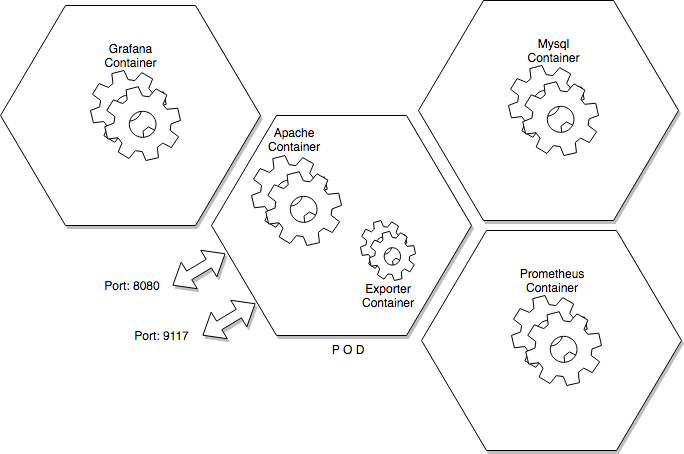
\includegraphics[scale=0.6]{SidecarDiagram.png}
  \label{fig:SidecarDiagram}
\end{figure}
\end{frame}

\begin{frame}[fragile]
  \frametitle{Apache status}
  Module to enable the output statistic of \emph{Apache}.

  \begin{figure}
    \begin{apachecode}
      <Location /server-status>
        SetHandler server-status
        Order deny,allow
        Allow from all
      </Location> ExtendedStatus On>
    \end{apachecode}
    \caption{status.conf}

    This module has to be copied in the \emph{/etc/apache2/mods-enabled/} directory.
  \end{figure}
\end{frame}

\begin{frame}[fragile]
  \frametitle{Dockerfile}
  The \emph{Dockerfile} includes the copy of the \emph{Apache} module\\
  Important to add the switching between \textit{root} and \textit{1001} user
  \begin{figure}
    \begin{dockercode}
      FROM ubuntu:latest
      USER root
      ...
      RUN a2enmod status
      COPY status.conf /etc/apache2/mods-enabled/
      EXPOSE 8080
      USER 1001
      CMD ["/usr/sbin/apache2ctl", "-DFOREGROUND"]
    \end{dockercode}
    \caption{Dockerfile}
  \end{figure}

\end{frame}

\begin{frame}[fragile]
  \frametitle{Secret Access}
  And because the credential of \emph{GITLAB}, we'll use the login/password based on the token initialized in our profile
  \begin{figure}
    \begin{yamlcode}
      apiVersion: v1
      kind: Secret
      metadata:
        name: gitlab-secret
        namespace: sidecar
      type: kubernetes.io/basic-auth
      data:
        username: c3Bpa2U=
        password: dmFsZW50aW5l
    \end{yamlcode}
    \caption{gitlab-secret.yaml}
  \end{figure}
\end{frame}

\begin{frame}[fragile]
  \frametitle{Secret Access}
  The \emph{username} and \emph{password} are encoded to Base64 format. Finally we load the new \emph{secret}
  \begin{bashcode}
    $ echo -n 'spike' | base64
    c3Bpa2U=
    $ echo -n 'valentine' | base64
    dmFsZW50aW5l
    $ oc create -f gitlab-secret.yaml
  \end{bashcode}
\end{frame}

\begin{frame}[fragile]
  \frametitle{New Project}
  It's time to create our new project \emph{sidecar}, similar to a namespace
  \begin{bashcode}
    $ oc new-project sidecar \
    --display-name='Side Car Project' \
    --description='Side Car Project'
  \end{bashcode}
\end{frame}

\begin{frame}[fragile]
  \frametitle{New Application}
  It's time to create our application
  \begin{bashcode}
    $ oc new-app https://gitlab.forge.orange-labs.fr/\
    laov6410/cdnselect.git --name sidecar
    $ oc set build-secret --source bc/sidecar gitlab-secret
    $ oc expose service sidecar
    $ oc get all name --selector app=sidecar
  \end{bashcode}
\end{frame}

\begin{frame}[fragile]
  \frametitle{Item To Modify}
  2 parts will be modified to adapted to our application
  \begin{itemize}
  \item DeploymentConfig
  \item Service
  \end{itemize}
\end{frame}

\begin{frame}[fragile]
  \frametitle{DeploymentConfig}
  We edit \emph{DeploymentConfig}
  \begin{bashcode}
    $ oc edit dc/sidecar
  \end{bashcode}
  and we add
  \begin{yamlcode}
    spec:
      containers:
      - name: apache-exporter
        image: previousnext/apache-exporter
        command: [ "apache_exporter", "-scrape_uri", \
        "http://127.0.0.1:8080/server-status/?auto" ]
        ports:
        - containerPort: 9117
  \end{yamlcode}
\end{frame}

\begin{frame}[fragile]
  \frametitle{Service}
  We edit \emph{service}
  \begin{bashcode}
    $ oc edit svc/sidecar
  \end{bashcode}

  \begin{yamlcode}
    spec:
      ...
      - name: 9117-tcp
        port: 9117
        protocol: TCP
        targetPort: 9117
  \end{yamlcode}
  9117 is The port related to \emph{exporter apache}
\end{frame}

\begin{frame}[fragile]
  \frametitle{Finally}
  Finally we create our new application from this \emph{yaml} file
  \begin{bashcode}
    $ oc get svc --selector "app=selector"
    NAME      TYPE        CLUSTER-IP      PORT(S)           
    selector  ClusterIP   172.30.127.98   8080/TCP,9117/TCP
    $ oc describe dc/sidecar
  \end{bashcode}
  Et voila...
\end{frame}
